	\section{Übersicht}
	\subsection{Architektur}
	Das System basiert auf dem Model-View-Controller(MVC)-Muster mit einer drei-Schichten-Architektur und einer durch JavaFX realisierten graphischen Benutzerschnittstelle.\\	
	 Beim MVC-Muster wird das System in die drei Komponenten Modell, Präsentation und Steuerung aufgeteilt.\\
	Das Modell (Model) enthält und verarbeitet die Daten, welche dann von der Präsentation (View) dargestellt werden. Die Steuerung (Controller) steuert den Ablauf und das Verhalten der Anwendung. Dafür werden Benutzereingaben auf Modeländerungen und Ausführung von Berechnungen abgebildet. Weiterhin informiert das Model direkt oder über den Controller die View über Änderungen am Model (z.B. Ergebnisse von Berechnungen) und sorgt damit für eine Anpassung bzw. Aktualisierung der View.\\
	In der hier verwendeten Architektur erfolgt die Kommunikation zwischen View und Model immer über den Controller. Dabei gibt es \texttt{FXController}-Komponenten, welche die Steuerung der View übernehmen, und \texttt{Controller}-Komponenten, welche als Schnittstelle zwischen den \texttt{FXControllern} und dem Model dienen.\\
	Dadurch kann das System in drei logische Schichten unterteilt werden, eine Daten-, eine Logik- und eine Benutzerschicht \ref{img:struktur}.
	%Diese Architektur ist durch Erweiterung bzw. einen Austausch der \textbf{Controller}-Komponenten auch in eine physisch getrennte drei-Schichten-Architektur überführbar.\\
		
	
	
	
	\begin{figure}
	\centering
	%\fbox{
	%\begin{subfigure}[t]{0.4\textwidth}
%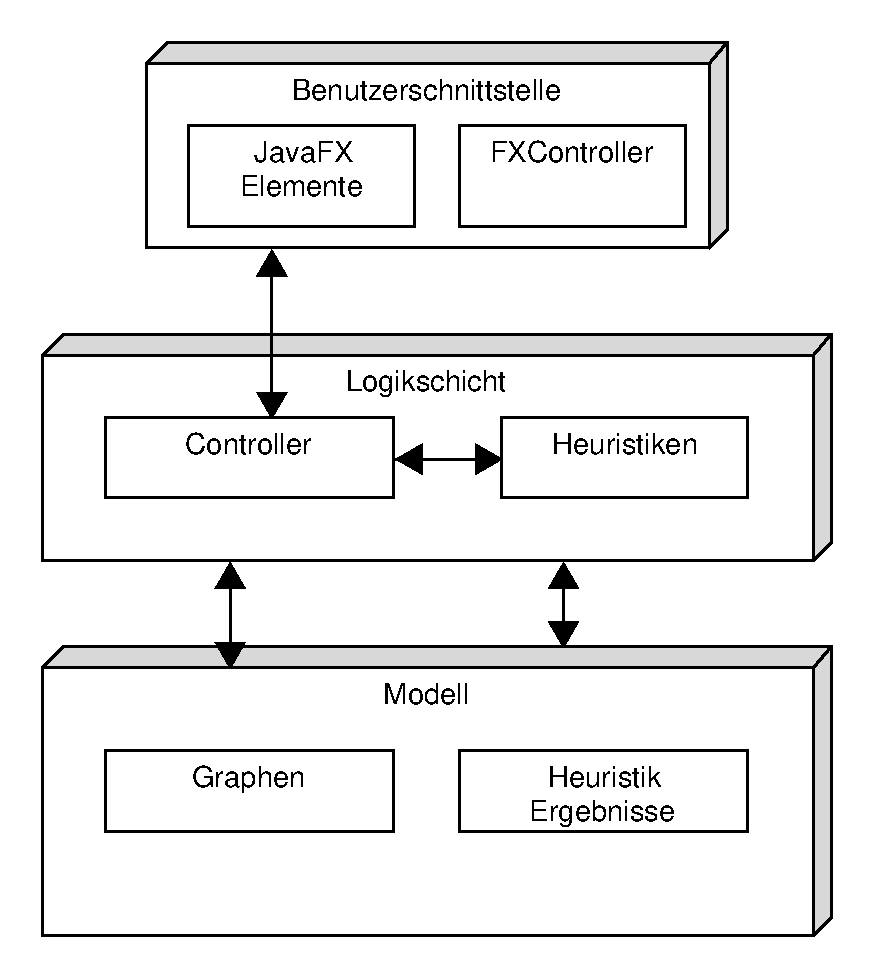
\includegraphics[height=2.8in]{struktur2.pdf}
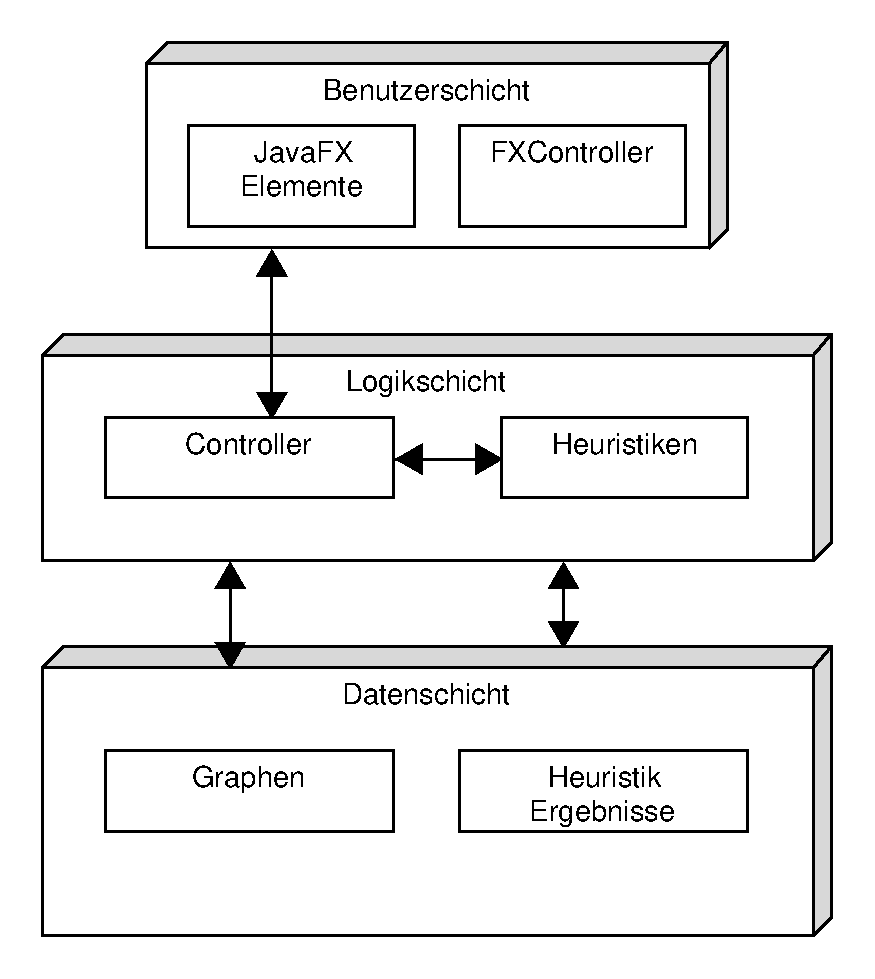
\includegraphics[height=2.8in]{abbildungen/struktur3.pdf}

%\subcaption{Darstellung als Schichtenarchitektur.}
%\end{subfigure}
	%\begin{subfigure}[t]{0.4\textwidth}
%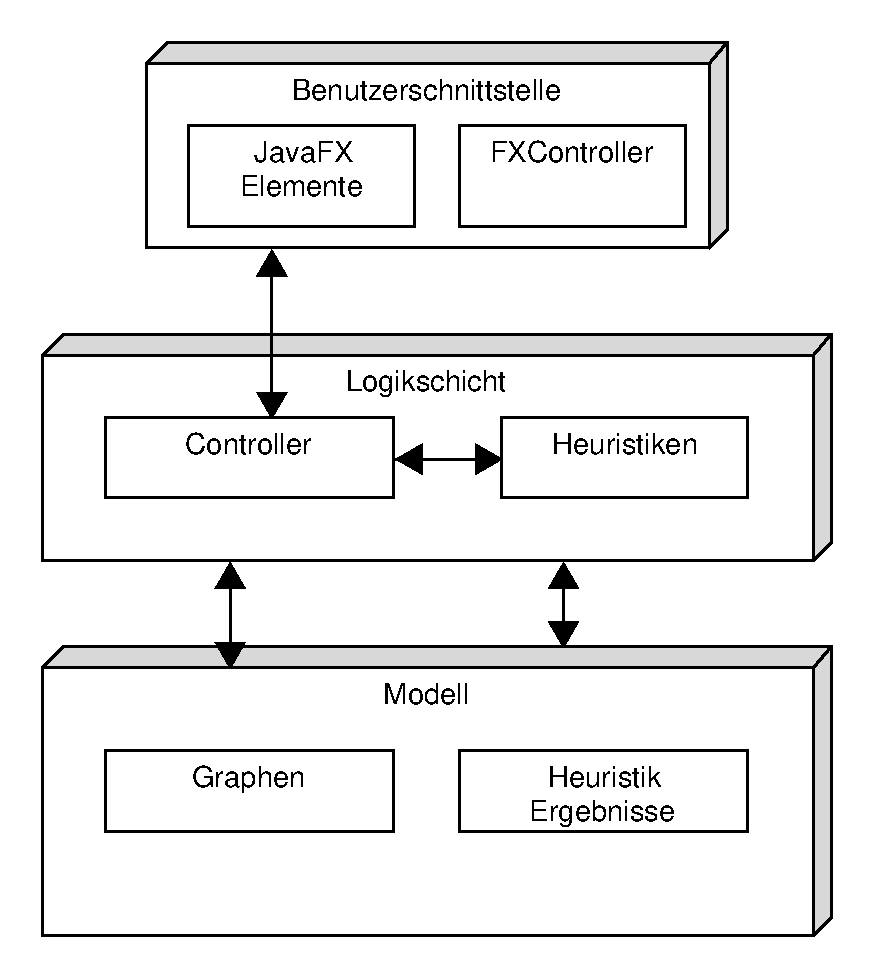
\includegraphics[height=2.8in]{struktur2.pdf}
%\subcaption{Model-View-Controller.}
%\end{subfigure}
%   }
	\caption{Die Architektur als drei-Schichtenmodell }
	\label{img:struktur}
\end{figure}

\subsection{Sequenzdiagramme}
Durch Benutzereingaben initiierte Aktionen werden durch das JavaFX-Framework an die entsprechenden \texttt{FXController} weitergeleitet. (TODO wie werden Controller und Aktionen verbunden?). Dieses wird in den folgenden Diagrammen deshalb nicht dargestellt, sondern nur die anschließenden Interaktionen.
\subsubsection{Heuristiken ausführen}
	Eine Benutzereingabe zum Ausführen der Ausgewählten Heuristiken wird durch den \texttt{FXTabController} verarbeitet und and den \texttt{TabController} weitergeleitet. Zu jeder ausgewählten Heuristik wird die Methode \mbox{\texttt{addToHeuristic}} aufgerufen. Diese erzeugt zuerst ein Objekt der entsprechenden Heuristik. Diese wird zum \texttt{DataPool}, welcher Graphen mit darauf auszuführenden Heuristiken enthält, hinzugefügt. Dabei wird beim Hinzufügen die Heuristik über die \texttt{applyTo}-Methode auf alle Graphen im \texttt{DataPool} angewandt.\\
	Ist die Anwendung aller Heuristiken abgeschlossen, wird eine Liste von Ergebnissen der Berechnungen vom Typ \texttt{HeuristicResult} vom \texttt{DataPool} zurückgegeben und über den \texttt{TabController} an den \texttt{FXTabController} weitergeleitet.
	
	\begin{figure}
	\centering
	%\fbox{	
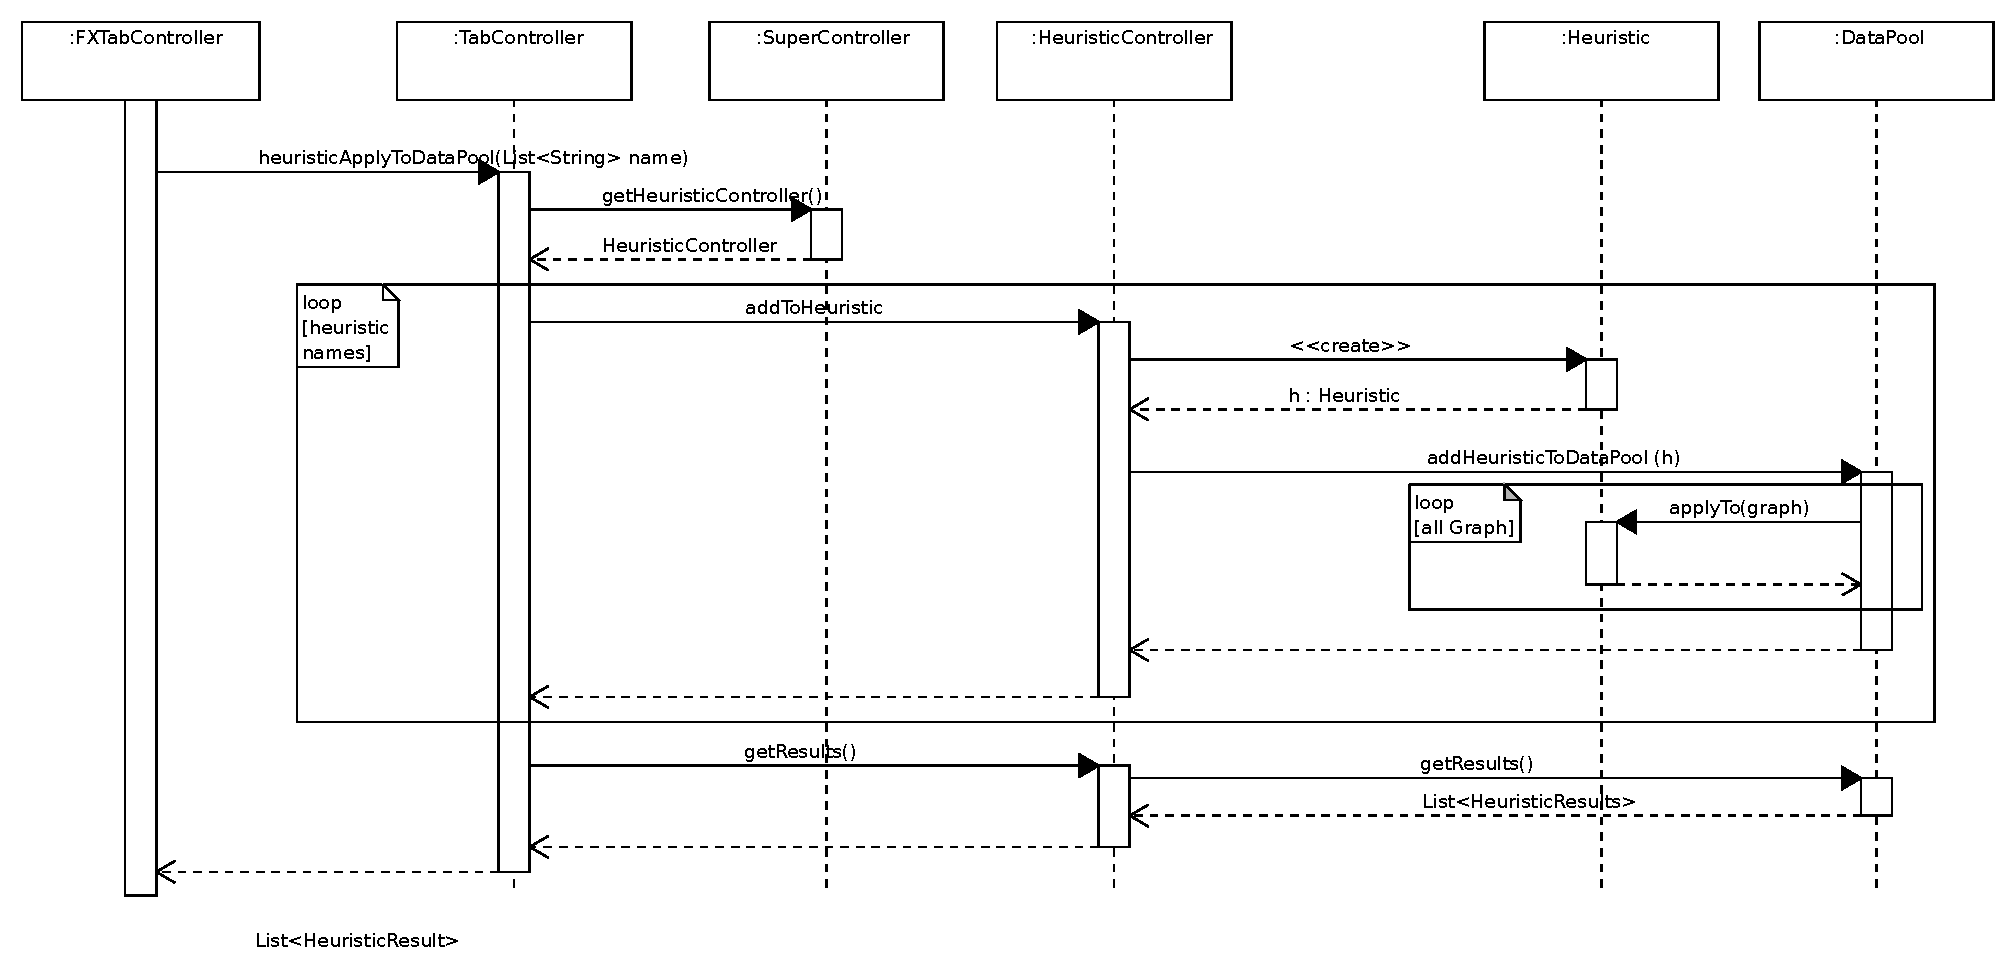
\includegraphics[width=\textwidth]{abbildungen/heuristik-seq.pdf}
\caption{Sequenzdiagramm zum Ausführen von Heuristiken }
	\label{img:heuristic-seq}
	\end{figure}
\subsubsection{Graphen generieren}
Eine Benutzereingabe zum Generieren von Graphen wird vom \texttt{FXGraphGeneratorController} verarbeitet. Dieser delegiert durch den Aufruf der Methode \texttt{generate} an den \texttt{GraphGeneratorController}. Hier wird für alle $n$ zu generierenden Graphen durch die Klasse \texttt{GraphBuilder} jeweils ein Objekt vom Typ \texttt{Graph} erzeugt und zu einem \texttt{DataPool} hinzugefügt. Jeder dieser Graphen wird anschließend durch die Klasse \texttt{GraphAdapter} in eine für die View benötigte Graphenstruktur umgewandelt.\\
Nach Generierung der Graphen wird ein neuer \texttt{TabController} erzeugt. Diesem wird der \texttt{DataPool} der neu generierten Graphen übergeben. Zum Schluss wird noch ein neuer \texttt{FXTabController} erzeugt, welcher für die Anzeige des Tabs für die generierten Graphen zuständig ist.

\begin{figure}
	\centering
	%\fbox{	
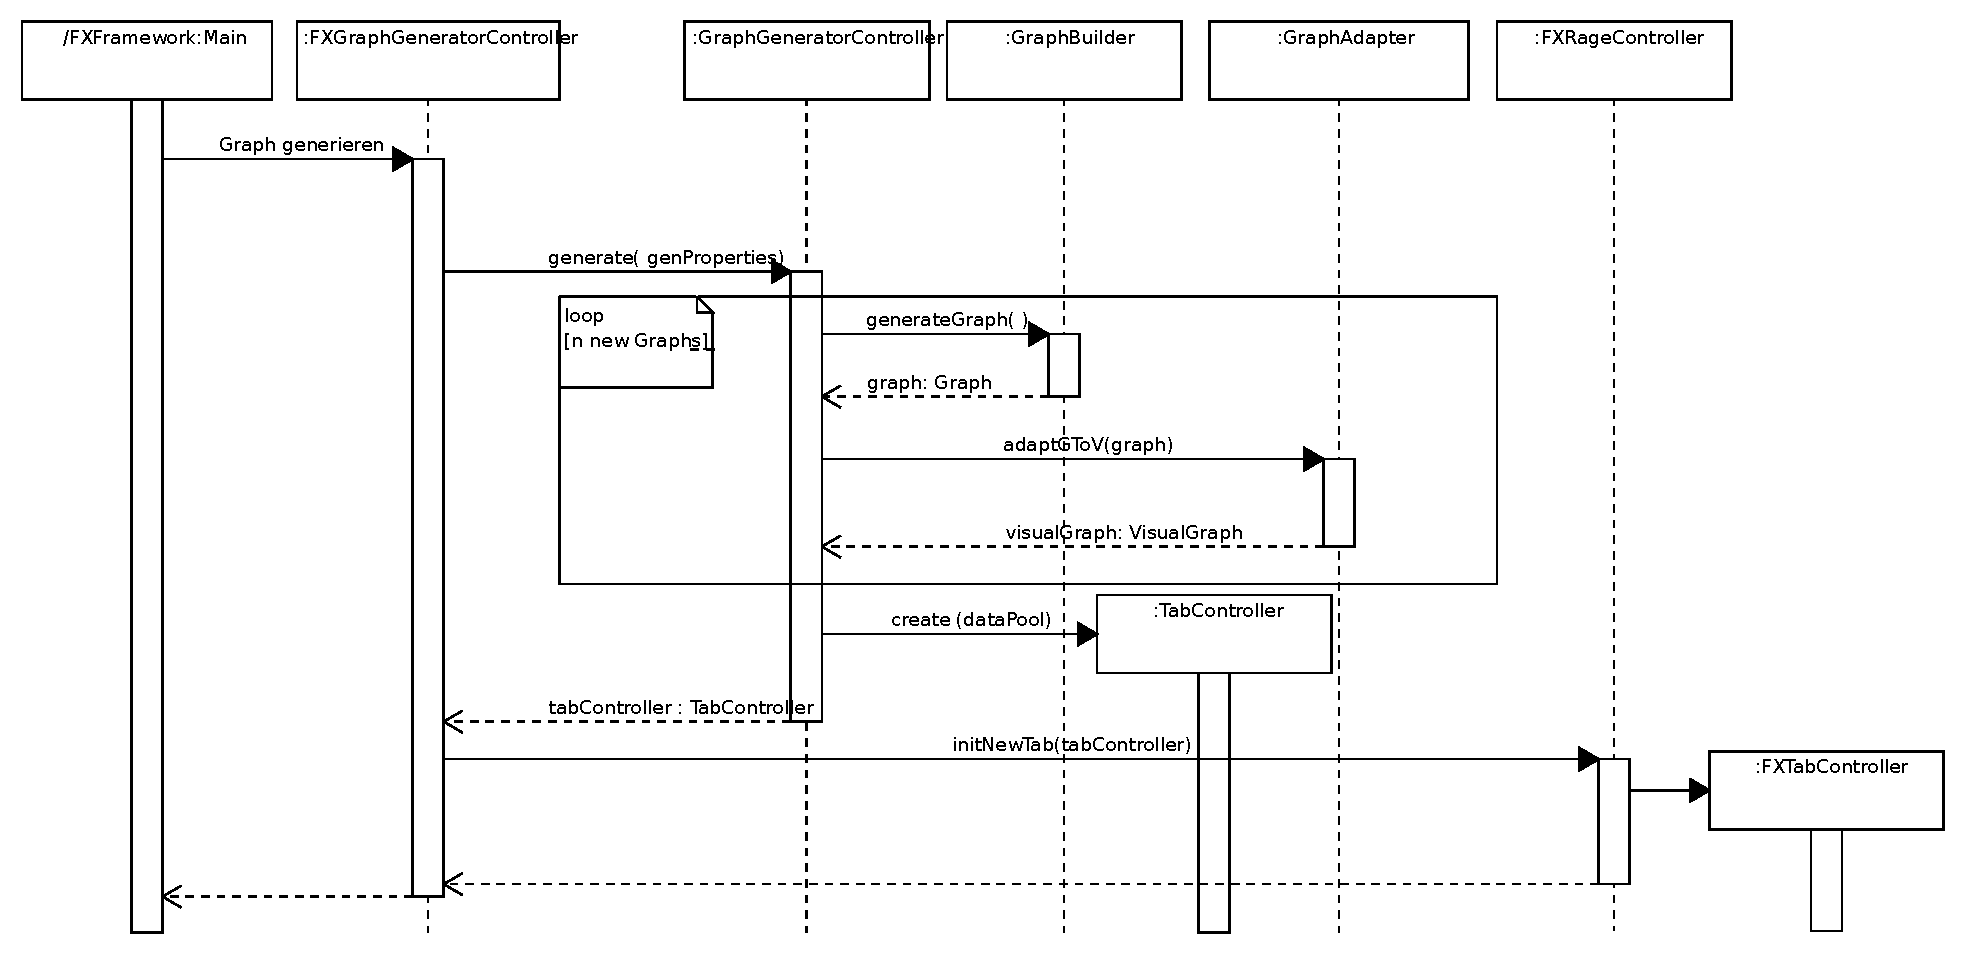
\includegraphics[width=\textwidth]{abbildungen/graphgen-seq.pdf}
\caption{Sequenzdiagramm zum Generieren von Graphen }
	\label{img:graphgen-seq}
	\end{figure}
	
	\subsubsection{Graphen modifizieren}
	Das Modifizieren von Graphen erfolgt über die Detailansicht des Graphen. Dafür wird zuerst ein \newline \texttt{FXDetailViewController} erzeugt. Bekommt dieser anschließend eine Benutzereingabe zum Modifizieren, dann wird ein \texttt{FXGraphEditorController}-Objekt erzeugt. Den dafür benötigten \texttt{GraphEditorConroller} erhält er über den Aufruf der Methode \texttt{getGEC} des \texttt{SuperControllers}.\\
	Anschließende Editierbefehle werden direkt an den \texttt{FXGraphEditorController} weitergeleitet und von diesem verarbeitet. Bei Abschluss des Editieren durch den Benutzer wird der modifizierte Graph als neuer Graph durch den \texttt{GraphEditorController} zum \texttt{DataPool} hinzugefügt.
\begin{figure}
	\centering
	%\fbox{	
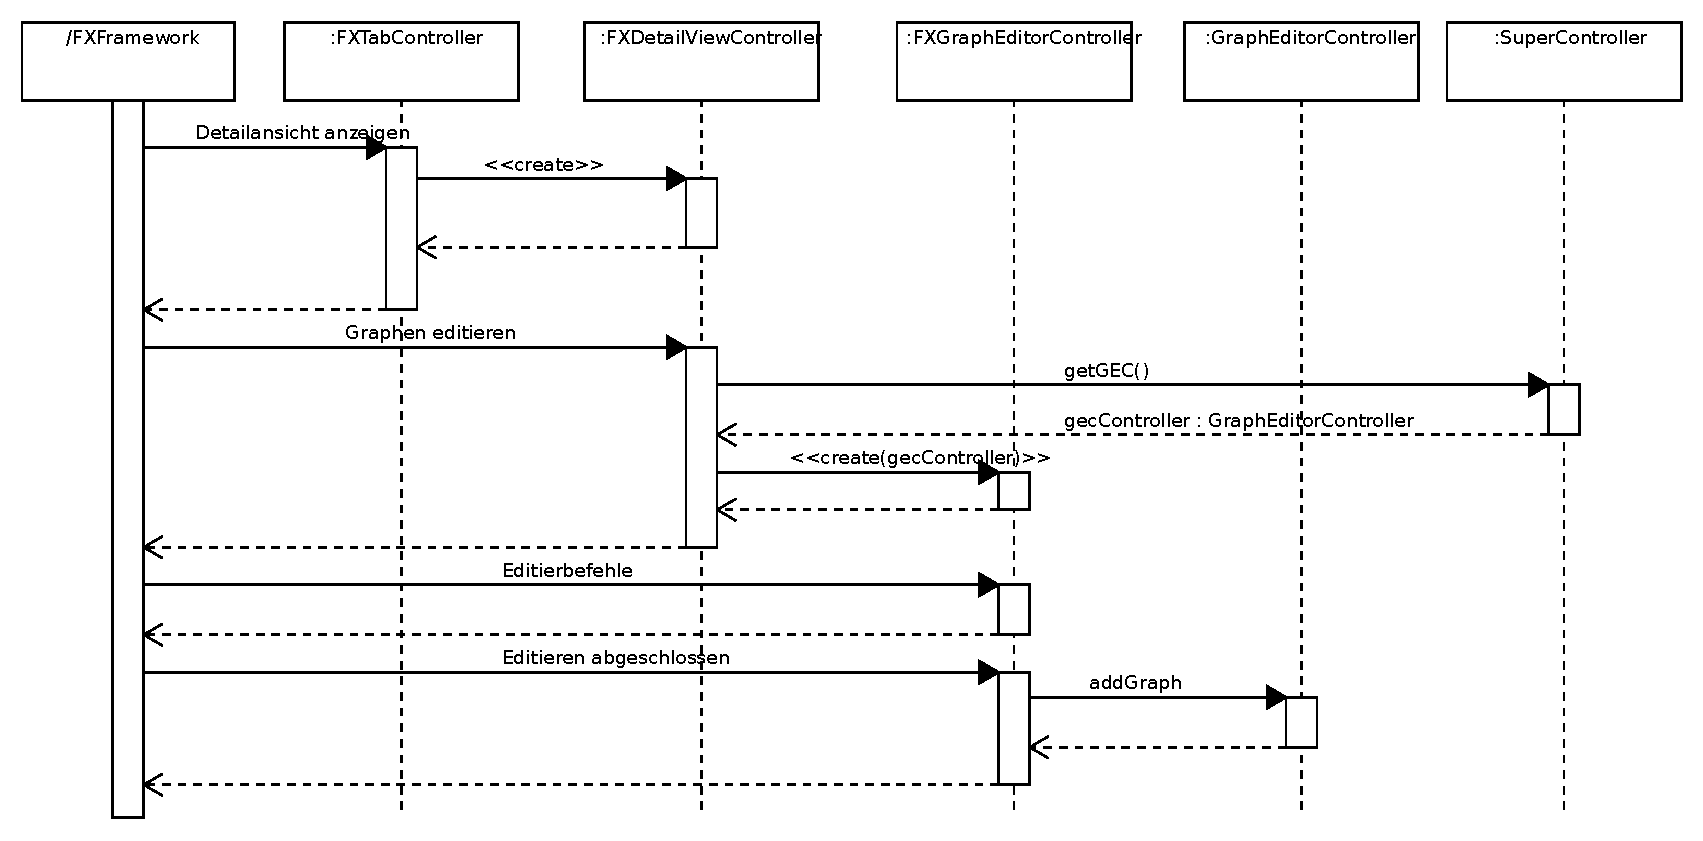
\includegraphics[width=\textwidth]{abbildungen/graphmod-seq.pdf}
\caption{Sequenzdiagramm zum Modifizieren von Graphen }
	\label{img:grapmod-seq}
	\end{figure}
	